% ============================================================
% Bai bao NCKH (mau SSRC / IEEEtran) - tieng Viet - BAN MOI (v2, du lieu sach)
% BIEN DICH: dung XeLaTeX (Overleaf: Menu -> Compiler -> XeLaTeX)
% Font: TeX Gyre Termes (tuong duong Times New Roman, co san tren Overleaf)
% ============================================================
\documentclass[10pt,journal,letterpaper]{IEEEtran}

\usepackage{fontspec}
\setmainfont{texgyretermes}[Extension=.otf,UprightFont=*-regular,BoldFont=*-bold,ItalicFont=*-italic,BoldItalicFont=*-bolditalic]
\usepackage{amsmath}
\usepackage{graphicx}
\usepackage{booktabs}
\usepackage{pgfplots}
\usetikzlibrary{arrows.meta,positioning}
\usepackage{url}
\Urlmuskip=0mu plus 1mu\relax
\pgfplotsset{compat=1.16}
\usepackage[top=0.7in,bottom=0.7in,left=0.65in,right=0.65in]{geometry}

\renewcommand{\figurename}{Hình}
\renewcommand{\tablename}{Bảng}
% Tieu de muc lon (\section) canh TRAI, thong nhat voi \subsection (IEEEtran mac dinh canh giua)
\makeatletter
\renewcommand\section{\@startsection{section}{1}{\z@}%
  {1.5ex plus 1.5ex minus 0.5ex}{0.7ex}{\normalfont\scshape\raggedright}}
\makeatother

\begin{document}

\title{Đánh giá phát hiện phương tiện giao thông Việt Nam có kiểm tra rò rỉ dữ liệu: so sánh YOLOv8s và Faster R-CNN trong miền và ngoài miền}

\author{[Họ và tên tác giả 1], [Họ và tên tác giả 2], [Họ và tên tác giả 3]\\
Nhóm 02, [Khoa/Trường]. Email: [email liên hệ]}

\markboth{Student Scientific Research Communication, Volume II, 2025}{}
\maketitle

% ------------------------------------------------------------
\begin{abstract}
Dữ liệu phương tiện giao thông Việt Nam đến từ nhiều camera, và các khung hình cùng video gần như giống hệt nhau, nên việc đánh giá mô hình phát hiện dễ lạc quan. Chúng tôi hợp nhất năm nguồn công khai, quy đổi về bốn lớp (xe máy, ô tô, xe buýt, xe tải) và chia theo video. Kiểm tra bổ sung trên bản chia đầu tiên cho thấy validation còn lẫn camera của tập huấn luyện; chúng tôi thay bằng một camera riêng, lọc dữ liệu huấn luyện rồi huấn luyện lại theo giao thức cố định, chọn checkpoint chỉ bằng validation sạch. Trên tập kiểm thử 1.500 ảnh, mô hình một giai đoạn YOLOv8s đạt mAP@0,5 là 0,7636 (thấp hơn bản chia cũ 2,94 điểm), so với 0,6408 của mô hình hai giai đoạn Faster R-CNN ResNet50-FPN, và nhanh hơn khoảng 4,6 lần về độ trễ mô hình. Trên bộ ảnh góc nhìn trên cao ngoài miền huấn luyện, mAP@0,5 là 0,5459. Trên bản chia cũ, chúng tôi còn báo cáo các cải tiến không hiệu quả (đầu phát hiện vật nhỏ, tăng độ phân giải, nhãn giả) và một khảo sát trọng số lớp cho mức cải thiện nhỏ (0,54 điểm), chưa tách được khỏi dao động giữa các lần chạy. Hạn chế: một lần huấn luyện cho mỗi cấu hình, kiểm thử chỉ có hai camera ban ngày, và kiểm tra camera chưa là bằng chứng tuyệt đối.
\end{abstract}

\begin{IEEEkeywords}
Phát hiện đối tượng, YOLOv8, Faster R-CNN, rò rỉ dữ liệu, phương tiện giao thông, đánh giá ngoài miền
\end{IEEEkeywords}

% ------------------------------------------------------------
\section{Giới thiệu}
Hệ thống camera giám sát giao thông tại các đô thị Việt Nam tạo ra lượng lớn hình ảnh có thể dùng để thống kê cơ cấu phương tiện, hỗ trợ quy hoạch và điều phối tín hiệu. Bài toán cốt lõi là phát hiện đối tượng đa lớp: xác định đồng thời vị trí và nhãn lớp của từng phương tiện trong khung hình. Các bộ phát hiện dựa trên mạng nơ-ron tích chập như YOLO~\cite{yolo} và Faster R-CNN~\cite{frcnn} thực hiện được cả hai yêu cầu này.

Dữ liệu giao thông Việt Nam có ba đặc điểm gây khó cho việc đánh giá. Thứ nhất, dữ liệu công khai (chủ yếu trên Roboflow Universe) đến từ nhiều camera với quy ước nhãn khác nhau, nên phải chuẩn hóa nhãn trước khi dùng chung. Thứ hai, các khung hình lấy từ cùng một video gần như giống hệt nhau. Nếu chia tập huấn luyện và kiểm thử theo khung hình, mô hình có thể ``ghi nhớ cảnh'' thay vì học khái niệm phương tiện, làm kết quả đánh giá lạc quan. Các phiên bản đầu của đề tài (V1--V4) chia theo khung hình nên có nguy cơ này; từ phiên bản V5 chúng tôi chuyển sang chia theo video. Thứ ba, phân bố lớp rất lệch: trên toàn bộ dữ liệu gộp (kể cả tập kiểm thử), xe máy chiếm khoảng 69\% số hộp, ô tô 19\%, xe tải 9\% và xe buýt 3\%, nên chỉ số trung bình mAP dễ che khuất chất lượng của các lớp thiểu số.

\textbf{Khoảng trống.} Trong phạm vi các công trình chúng tôi tiếp cận được, việc báo cáo kết quả phát hiện phương tiện Việt Nam thường thiếu bốn yếu tố cùng lúc: (i) nêu rõ cách kiểm soát rò rỉ dữ liệu và giới hạn của cách kiểm soát đó; (ii) so sánh bộ phát hiện một giai đoạn và hai giai đoạn dưới cùng dữ liệu, cùng phần cứng; (iii) đánh giá ngoài miền huấn luyện; (iv) báo cáo AP theo từng lớp và cả các cải tiến không hiệu quả. Nhận định này cần được đối chiếu thêm với tài liệu khác. Chúng tôi không đề xuất một kiến trúc hay hàm mất mát mới; đóng góp của bài là một đánh giá có phương pháp và minh bạch về phạm vi.

\textbf{Đóng góp.} Bài báo có bốn đóng góp:
\begin{enumerate}
\item Xây dựng bộ dữ liệu V5+ hợp nhất từ năm nguồn công khai về schema bốn lớp, chia tập theo video, kèm kiểm tra toàn vẹn nhãn và giao nhau giữa các tập. Chúng tôi chỉ ra rằng bản chia đầu còn lẫn camera giữa train và validation, đề xuất bản chia sạch (validation là camera riêng) cùng giao thức huấn luyện cố định, và nêu rõ giới hạn của các kiểm tra này (mục~\ref{sec:data}).
\item So sánh có đối chứng YOLOv8s với Faster R-CNN ResNet50-FPN trên cùng tập kiểm thử và cùng GPU, về độ chính xác (kể cả theo từng lớp) và tốc độ.
\item Đánh giá ngoài miền trên bộ ảnh góc nhìn trên cao (VN Aerial) và công bố các cải tiến không hiệu quả (đầu phát hiện P2, tăng độ phân giải, curriculum, pseudo-label), thử trên bản chia cũ.
\item Khảo sát sơ bộ trọng số lớp (\texttt{cls\_pw}) của Ultralytics như một trong các cải tiến (trên bản chia cũ), báo cáo mức cải thiện theo từng lớp cùng các giới hạn của nó.
\end{enumerate}

% ------------------------------------------------------------
\section{Công trình liên quan}
\subsection{Phát hiện đối tượng}
Mạng nơ-ron tích chập học đặc trưng trực tiếp từ ảnh thay cho các bộ mô tả thủ công. Mạng phần dư ResNet~\cite{resnet} dùng kết nối tắt để huấn luyện mạng sâu mà không suy biến gradient và thường là xương sống (backbone) của các bộ phát hiện; mạng kim tự tháp đặc trưng FPN~\cite{fpn} kết hợp đặc trưng nhiều tỷ lệ để phát hiện vật có kích thước khác nhau.

Faster R-CNN~\cite{frcnn} là đại diện của hướng hai giai đoạn: mạng đề xuất vùng (RPN) dùng chung đặc trưng tích chập với mạng phát hiện sinh các ứng viên, sau đó đầu phân loại và hồi quy tinh chỉnh từng ứng viên. Hướng một giai đoạn bỏ bước đề xuất vùng: YOLO~\cite{yolo} xử lý toàn ảnh trong một lượt và dự đoán trực tiếp hộp và lớp, còn SSD~\cite{ssd} dự đoán trên các hộp mặc định ở nhiều độ phân giải đặc trưng. Hai hướng này đổi chác tốc độ lấy độ chính xác theo cách khác nhau, nên chúng tôi so sánh cả hai trên cùng dữ liệu.

YOLOv8 là phiên bản do Ultralytics duy trì, có đầu tách nhánh phân loại và hồi quy, thiết kế không neo (anchor-free), và hàm mất mát kết hợp mất mát hộp với Distribution Focal Loss~\cite{yolov8docs}. Chúng tôi chọn biến thể small (YOLOv8s) làm mô hình chính vì cân bằng giữa tốc độ và độ chính xác, đồng thời vừa với bộ nhớ 12~GB của GPU thí nghiệm; Faster R-CNN ResNet50-FPN là mô hình đối chứng.

\subsection{Mất cân bằng lớp trong phát hiện đối tượng}
Các hướng chính là đặt lại trọng số mất mát và lấy mẫu lại. Class-balanced loss gán trọng số theo số mẫu hiệu dụng của mỗi lớp~\cite{cbloss}; focal loss giảm đóng góp của mẫu dễ~\cite{focal}. Với phân bố đuôi dài trên LVIS, Equalization Loss~\cite{eql} và Seesaw Loss~\cite{seesaw} điều chỉnh gradient của các lớp hiếm. Phan và Yamamoto~\cite{phan} so sánh các biến thể cross-entropy có trọng số trên BDD100K~\cite{bdd}, tập dữ liệu lái xe có Car chiếm ưu thế, và báo cáo cải thiện AP theo từng lớp. Ngược lại, Crasto~\cite{crasto} báo cáo rằng lấy mẫu và đặt lại trọng số không giúp được YOLOv5 trên tập con COCO 10 lớp có phân bố đuôi dài. Hai kết quả trái chiều này cho thấy hiệu quả của đặt lại trọng số với bộ phát hiện một giai đoạn chưa chắc chắn; vì vậy chúng tôi chỉ thử một cấu hình trọng số lớp cho YOLOv8 như một trong các cải tiến và báo cáo đúng mức hiệu quả của nó.

\subsection{Dữ liệu giao thông}
Các bộ dữ liệu như UA-DETRAC~\cite{detrac} và BDD100K~\cite{bdd} được dùng rộng rãi cho phương tiện. Cả hai được thu thập ở nước ngoài, với tỷ lệ xe máy thấp và tổ chức giao thông khác Việt Nam, nên số liệu trên các bộ này không thay thế được đánh giá trên dữ liệu trong nước. COCO~\cite{coco} chủ yếu đóng vai trò nguồn trọng số tiền huấn luyện trong học chuyển giao. Dữ liệu công khai về phương tiện Việt Nam chủ yếu được phát hành trên Roboflow Universe từ nhiều camera với quy ước nhãn khác nhau, vì vậy cần chuẩn hóa nhãn và kiểm soát cách chia tập trước khi huấn luyện.
% TODO: bo sung trich dan cac bo du lieu giao thong Viet Nam da cong bo (vi du Da Nang CCTV 2026,
%       UIT-VinaDeveS22) sau khi doc toan van; chua dua vao vi chua kiem chung chi tiet.

\subsection{Rò rỉ dữ liệu khi chia tập theo khung hình}
Camera cố định quay 25--30 khung hình mỗi giây; hai khung hình liên tiếp có nền, vạch kẻ và ánh sáng gần như giống nhau, chỉ khác vị trí phương tiện vài điểm ảnh. Chia ngẫu nhiên theo khung hình đặt các bản sao gần như y hệt vào cả tập huấn luyện lẫn kiểm thử, nên điểm kiểm thử đo khả năng ``nhớ cảnh'' hơn là khả năng khái quát. Chia theo video là bước kiểm soát cần thiết, nhưng chưa đủ: hai video khác nhau vẫn có thể quay cùng một camera và cùng cảnh, nên đánh giá độc lập thực sự đòi hỏi gom mọi video của cùng camera vào một tập. Nhận định này là kết luận từ kiểm tra dữ liệu của chúng tôi (mục~\ref{sec:data}) chứ không dẫn từ một công trình cụ thể.

% ------------------------------------------------------------
\section{Dữ liệu}\label{sec:data}
\subsection{Nguồn dữ liệu và schema bốn lớp}
Bộ V5+ hợp nhất năm nguồn công khai, đều theo giấy phép CC BY 4.0 trên Roboflow Universe (Bảng~\ref{tab:src}). Nhãn của mọi nguồn được quy đổi về bốn lớp: xe máy (motorcycle), ô tô con (car), xe buýt (bus) và xe tải (truck, gồm cả container). Các lớp khác như xe đạp, xe ba gác, xe van hoặc người bị loại bỏ thay vì gộp sang lớp gần nhất, nhằm tránh học nhầm hình dáng. Ảnh chỉ còn nhãn bị loại được giữ lại như ảnh nền. Tổng cộng có 10.203 ảnh từ 368 camera hoặc bối cảnh, chứa 87.460 hộp giới hạn.

\begin{table*}[!t]
\caption{Các nguồn dữ liệu của bộ V5+ (số ảnh sau lấy mẫu và số hộp theo lớp)}
\label{tab:src}
\centering
\footnotesize
\begin{tabular}{lrrrrr}
\toprule
Nguồn & Ảnh & Xe máy & Ô tô & Xe buýt & Xe tải \\
\midrule
SOICT 2024 (camera ngày TP.HCM) & 3.379 & 49.691 & 11.260 & 1.779 & 4.605 \\
SOICT Night (camera đêm TP.HCM) & 1.385 & 4.751 & 2.578 & 748 & 844 \\
Vehicle Vietnam-CanTho & 725 & 2.152 & 1.710 & 19 & 140 \\
Vietnamese Vehicle v3 & 310 & 471 & 570 & 68 & 361 \\
Vietnam Vehicles v10 (snapshot CCTV) & 4.404 & 3.336 & 265 & 253 & 1.859 \\
\midrule
\textbf{Tổng V5+} & \textbf{10.203} & \textbf{60.401} & \textbf{16.383} & \textbf{2.867} & \textbf{7.809} \\
Tỷ lệ số hộp & & 69\% & 19\% & 3\% & 9\% \\
\bottomrule
\end{tabular}
\end{table*}

\subsection{Chia tập và kiểm soát rò rỉ}
\textbf{Bản chia đầu (``bản chia cũ'').} Tập huấn luyện gồm 7.237 ảnh (gồm toàn bộ 4.404 ảnh của Vietnam Vehicles v10), tập validation 1.466 ảnh và tập kiểm thử 1.500 ảnh. Tập kiểm thử chỉ gồm hai camera ban ngày của SOICT 2024 (cam\_09 với 1.000 ảnh và cam\_10 với 500 ảnh). Video ngày được lấy mẫu mỗi 5 khung hình, video đêm mỗi 10 khung hình; ảnh snapshot được giữ nguyên. Chúng tôi chia theo \texttt{video\_id} suy ra từ tên tệp; kiểm tra theo quy tắc này không thấy giao nhau giữa các tập.

Kiểm tra bổ sung cho thấy quy tắc này \emph{chưa đủ}: 466 trong 1.466 ảnh validation (toàn bộ thuộc video Cần Thơ) cùng camera với video huấn luyện, và có 102 cặp ảnh gần trùng giữa huấn luyện và validation. Bốn video Cần Thơ (hai ở huấn luyện, hai ở validation) là cùng một camera: độ tương quan ảnh nền đạt 0,98 và 0,76, so với mức 0,73 trở lên của các cặp cùng video. Hệ quả là việc chọn checkpoint và dừng sớm theo validation cũ lạc quan. Tập kiểm thử không bị ảnh hưởng: ảnh gần nhất giữa kiểm thử và huấn luyện cách xa (khoảng cách mã băm 12, tương quan ảnh nền không quá 0,35).

\textbf{Bản chia sạch.} Chúng tôi (i) thay validation bằng camera \texttt{soict24\_cam\_07} (1.000 ảnh, camera riêng), bỏ phần Cần Thơ khỏi validation và không chuyển sang huấn luyện; (ii) giữ nguyên tập kiểm thử; (iii) lọc 4.824 ảnh v10 còn 4.136 ảnh bằng bốn quy tắc cố định trước khi huấn luyện: bỏ ảnh có xe ba gác (529 ảnh, vì schema không có lớp này), gộp ảnh trùng thật cùng camera (14), bỏ ảnh có xe chưa gán nhãn theo bộ phát hiện COCO (144) và bỏ nhãn lỗi (1). Tập huấn luyện sạch gồm 6.969 ảnh (2.833 ảnh V5 và 4.136 ảnh v10); Bảng~\ref{tab:split} so sánh hai bản chia, Bảng~\ref{tab:cleanbox} cho số hộp theo lớp. Trong tập huấn luyện sạch, xe máy chiếm 51\%, ô tô 23\%, xe tải 19\% và xe buýt 6\% số hộp, ít lệch hơn so với 69/19/9/3\% của toàn bộ dữ liệu gộp vì tập kiểm thử có rất nhiều xe máy.

Kết quả kiểm tra bản chia sạch: không có cặp ảnh nào có khoảng cách mã băm không quá 5 giữa huấn luyện với validation hay kiểm thử; độ tương quan ảnh nền giữa camera validation/kiểm thử và camera huấn luyện gần nhất là 0,5059 (kiểm thử), 0,4748 (validation), thấp hơn mức 0,6774 của cặp đối chứng dương cùng camera. Đây là kiểm tra \emph{dựa trên mã băm ảnh và ảnh nền}, không phải bằng chứng tuyệt đối rằng hai tập không chia sẻ camera. Giới hạn khác: ảnh v10 chiếm 59\% tập huấn luyện sạch nhưng khác miền (ảnh chụp vi phạm, 1--3 xe mỗi ảnh, so với khoảng 33 hộp mỗi ảnh của kiểm thử) và khoảng 83\% trong đó có khung hay thẻ theo dõi vẽ sẵn lên ảnh.

\begin{table}[!t]
\caption{Hai bản chia dữ liệu (số ảnh)}
\label{tab:split}
\centering
\footnotesize
\begin{tabular}{lrrr}
\toprule
Bản chia & Huấn luyện & Validation & Kiểm thử \\
\midrule
Cũ & 7.237 & 1.466 (lẫn camera) & 1.500 \\
Sạch & 6.969 & 1.000 (cam\_07) & 1.500 \\
\bottomrule
\end{tabular}
\end{table}

\begin{table}[!t]
\caption{Số hộp theo lớp của bản chia sạch}
\label{tab:cleanbox}
\centering
\footnotesize
\begin{tabular}{lrrrr}
\toprule
Tập & Xe máy & Ô tô & Xe buýt & Xe tải \\
\midrule
Huấn luyện & 13.168 & 5.880 & 1.630 & 4.915 \\
Validation & 5.852 & 1.654 & 447 & 1.913 \\
\bottomrule
\end{tabular}
\end{table}

Để đo khả năng tổng quát hóa ngoài miền, chúng tôi dùng bộ VN Aerial gồm 486 ảnh validation và 149 ảnh kiểm thử chụp từ góc nhìn trên cao; so khớp MD5 xác nhận không có ảnh nào trùng với V5+.

% ------------------------------------------------------------
\section{Phương pháp}
\subsection{Giao thức huấn luyện sạch}
Mô hình chính của bài là YOLOv8s~\cite{yolov8docs}. Để kết quả không phụ thuộc vào validation bị rò rỉ, mô hình được huấn luyện trên bản chia sạch theo một giao thức cố định: khởi tạo từ trọng số COCO~\cite{coco} (không warm-start từ checkpoint đã chọn bằng validation cũ), độ phân giải $960\times960$, batch 16, 60 epoch, \emph{không dừng sớm}, tối ưu SGD với tốc độ học $0{,}01$ giảm cosine, mixup $0{,}15$, xoay $\pm5^{\circ}$, \texttt{close\_mosaic}$=10$, hạt giống 42. Checkpoint được chọn \emph{chỉ} theo validation sạch (cam\_07); tập kiểm thử được chạy đúng một lần sau khi huấn luyện xong, và không chỉnh quy tắc làm sạch hay siêu tham số sau khi xem kết quả kiểm thử. Các siêu tham số còn lại giữ mặc định của Ultralytics.

\subsection{Mô hình đối chứng hai giai đoạn}
Faster R-CNN ResNet50-FPN~\cite{tvfrcnn} khởi tạo từ COCO, huấn luyện 30 epoch bằng SGD, ảnh được đưa về kích thước 800/1.333. Mô hình này được huấn luyện trên bản chia cũ (trước khi có bản sạch) với một hạt giống không cố định. Vì tập kiểm thử không đổi giữa hai bản chia, so sánh trên tập kiểm thử vẫn hợp lệ, nhưng chúng tôi chưa huấn luyện lại nó trên bản sạch.

\subsection{Theo vết và đếm phương tiện}
Để dùng bộ phát hiện cho thống kê cơ cấu giao thông, chúng tôi ghép nó với bộ theo vết ByteTrack~\cite{bytetrack}. ByteTrack liên kết các phát hiện giữa các khung hình bằng độ chồng lấp IoU, ghép trước các phát hiện có độ tin cậy cao rồi mới ghép các phát hiện độ tin cậy thấp với những vết chưa được gán, và dùng bộ lọc Kalman để dự đoán vị trí khi bị che ngắn. Đầu ra là một mã định danh (ID) bền vững cho mỗi phương tiện.

Phép đếm dựa trên giao cắt đoạn thẳng. Người dùng đặt một hoặc nhiều vạch ảo và chọn hướng đếm. Với mỗi ID, hệ thống lưu tâm hộp ở khung hình trước; nếu đoạn nối tâm cũ với tâm mới cắt vạch, hệ thống ghi một sự kiện đếm gồm khung hình, tên vạch, hướng (xác định bằng dấu tích có hướng), ID và lớp. Mỗi cặp (vạch, ID) chỉ được đếm một lần, nên xe tấp vào lề rồi chạy ra không bị đếm hai lần. Kết quả xuất ra tệp CSV sự kiện và video chú thích. Sai số đếm được đo bằng sai số tuyệt đối trung bình theo lớp (MAE) và sai số phần trăm của tổng số lượt đếm. Hình~\ref{fig:pipe} tóm tắt quy trình.

\begin{figure}[!t]
\centering
\begin{tikzpicture}[node distance=0.35cm, every node/.style={font=\scriptsize},
  box/.style={draw, rounded corners=2pt, minimum height=0.95cm, text width=1.45cm, align=center, inner sep=2pt},
  arr/.style={-{Stealth[length=4pt]}, thick}]
\node[box] (v) {Video\\(khung hình)};
\node[box, right=of v] (d) {YOLOv8s\\hộp và lớp};
\node[box, right=of d] (k) {ByteTrack\\gán ID};
\node[box, right=of k] (c) {Vạch ảo\\đếm lượt};
\draw[arr] (v) -- (d); \draw[arr] (d) -- (k); \draw[arr] (k) -- (c);
\node[below=0.3cm of c, text width=3.6cm, align=center] (o) {CSV sự kiện và video chú thích};
\draw[arr] (c) -- (o);
\end{tikzpicture}
\caption{Quy trình phát hiện, theo vết và đếm phương tiện.}
\label{fig:pipe}
\end{figure}

\subsection{Chỉ số đánh giá}
Chúng tôi báo cáo Precision, Recall, mAP@0,5, mAP@0,5:0,95 và AP@0,5 theo từng lớp trên 1.500 ảnh kiểm thử. YOLO được đánh giá bằng \texttt{model.val()} của Ultralytics (FP16), Faster R-CNN bằng \texttt{pycocotools} với cùng quy ước bốn lớp; hai bộ đánh giá có thể lệch nhau chút ít. Do tính ngẫu nhiên của suy luận FP16, chênh lệch dưới $0{,}003$ giữa các lần đánh giá lại cùng một checkpoint được coi là trùng khớp. Số TP, FP và FN theo lớp được đếm ở ngưỡng tin cậy $0{,}25$, NMS IoU $0{,}7$ và ghép hộp với IoU $\ge0{,}5$. Kích thước hộp theo chuẩn COCO~\cite{coco}: nhỏ ($<32^2$ pixel), vừa ($32^2$--$96^2$) và lớn ($>96^2$).

\subsection{Thử nghiệm bổ sung trên bản chia cũ}
Trước khi có bản chia sạch, chúng tôi đã huấn luyện một số cải tiến trên bản chia cũ. Chúng được giữ lại để báo cáo các kết quả không hiệu quả, nhưng checkpoint của chúng được chọn theo validation còn lẫn camera, nên chỉ nên xem là so sánh tương đối. Cơ sở là YOLOv8s khởi tạo từ COCO, tối đa 40 epoch, batch 6, tốc độ học $0{,}005$ với lịch cosine, mixup $0{,}1$ (\emph{cơ sở cũ}). Bốn cải tiến chạy trên cơ sở cũ: (i) tăng cường không gian mạnh hơn ($\texttt{scale}=0{,}7$, $\texttt{translate}=0{,}15$), gọi là \texttt{p4\_scale}; (ii) tăng độ phân giải lên 1.280 (\texttt{p4\_imgsz1280}); (iii) thêm đầu phát hiện bước nhảy 4 cho vật nhỏ (\texttt{r\_p2}); (iv) curriculum độ phân giải 960 rồi 1.280 (\texttt{r\_progressive}). Ngoài ra, chúng tôi thử một cấu hình đặt trọng số lớp (\emph{YOLOv8s-CW}) với siêu tham số \texttt{cls\_pw} của Ultralytics.

Ultralytics (phiên bản 8.4.126) tính trọng số cho từng lớp từ số thực thể của lớp đó trong tập huấn luyện~\cite{ultraloss}. Gọi $n_c$ là số thực thể của lớp $c$ và $\gamma$ là \texttt{cls\_pw}, trọng số được chuẩn hóa để trung bình bốn lớp bằng 1:
\begin{equation}
w_c=\frac{(1/n_c)^{\gamma}}{\frac{1}{4}\sum_{k=1}^{4}(1/n_k)^{\gamma}},\qquad
\mathcal{L}_{\text{cls}}=\sum_{c} w_c\,\ell^{\text{BCE}}_c .
\end{equation}
Chỉ mất mát phân loại (BCE) được nhân trọng số; mất mát hộp và DFL không đổi. Với $\gamma=0{,}5$ trên tập huấn luyện của bản chia cũ, bốn trọng số là $0{,}571$ (xe máy), $0{,}860$ (ô tô), $1{,}629$ (xe buýt) và $0{,}940$ (xe tải). YOLOv8s-CW được tinh chỉnh tối đa 15 epoch từ checkpoint cơ sở cũ với tốc độ học $0{,}001$ và dừng sớm tại epoch 10 (checkpoint tốt nhất ở epoch 2).

% ------------------------------------------------------------
\section{Kết quả thực nghiệm}
Mô hình sạch được huấn luyện và đánh giá trên một GPU NVIDIA RTX 3500 Ada Laptop 12 GB, PyTorch 2.5.1, Ultralytics 8.4.142; các thử nghiệm bổ sung trên bản chia cũ chạy trên cùng GPU với PyTorch 2.7.1 và Ultralytics 8.4.126. Mỗi cấu hình chỉ được huấn luyện \emph{một lần} với một hạt giống ngẫu nhiên, nên chúng tôi không có khoảng tin cậy.

\subsection{Kết quả chính theo giao thức sạch}
Bảng~\ref{tab:clean} báo cáo YOLOv8s theo giao thức ở mục~IV-A; Bảng~\ref{tab:cleancls} cho AP theo lớp. Trên tập kiểm thử, YOLOv8s đạt mAP@0,5 là 0,7636, hơn Faster R-CNN (0,6408) 12,28 điểm và hơn YOLOv8s COCO không huấn luyện lại (0,4514) 31,22 điểm. AP của xe tải thấp nhất (0,6347), AP của ô tô cao nhất (0,8434). Checkpoint tốt nhất được chọn ở epoch 45 theo validation sạch, với mAP@0,5 trên validation là 0,8392; con số này cao hơn kiểm thử vì validation và kiểm thử là các camera khác nhau, có độ khó khác nhau. Đánh giá lại cùng checkpoint trên kiểm thử ở FP16 cho 0,7630, lệch 0,0006, nằm trong ngưỡng dao động 0,003; bảng dùng số của lần chạy kiểm thử chính thức. Hình~\ref{fig:curve} cho thấy mAP trên validation tăng nhanh trong khoảng 20 epoch đầu, đạt đỉnh quanh epoch 45 rồi dao động nhẹ khi mất mát huấn luyện tiếp tục giảm.

\begin{figure}[!t]
\centering
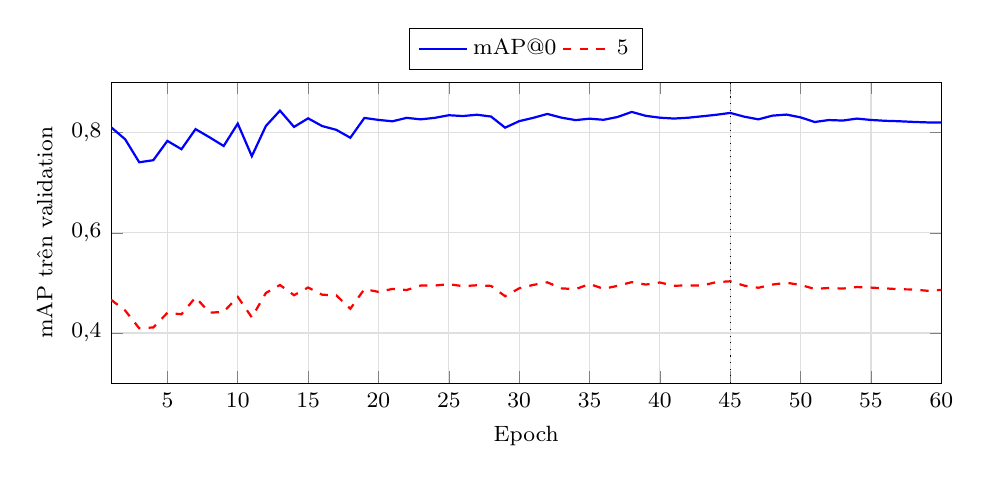
\begin{tikzpicture}
\begin{axis}[width=\columnwidth, height=5.4cm, xlabel={Epoch}, xlabel style={font=\footnotesize},
  ylabel={mAP trên validation}, ylabel style={font=\footnotesize}, tick label style={font=\footnotesize},
  xmin=1, xmax=60, ymin=0.3, ymax=0.9,
  legend style={font=\footnotesize, at={(0.5,1.04)}, anchor=south, legend columns=2},
  yticklabel style={/pgf/number format/.cd, use comma, fixed, precision=1}, grid=major, grid style={gray!25}]
\addplot[thick, blue, no markers] coordinates {(1,0.8106) (2,0.7866) (3,0.7407) (4,0.7449) (5,0.7834) (6,0.7668) (7,0.8069) (8,0.7905) (9,0.7732) (10,0.8179) (11,0.7529) (12,0.8132) (13,0.8438) (14,0.8113) (15,0.8284) (16,0.8130) (17,0.8055) (18,0.7897) (19,0.8292) (20,0.8253) (21,0.8225) (22,0.8294) (23,0.8264) (24,0.8294) (25,0.8346) (26,0.8330) (27,0.8356) (28,0.8320) (29,0.8098) (30,0.8228) (31,0.8294) (32,0.8372) (33,0.8298) (34,0.8249) (35,0.8277) (36,0.8255) (37,0.8312) (38,0.8412) (39,0.8334) (40,0.8297) (41,0.8280) (42,0.8296) (43,0.8325) (44,0.8355) (45,0.8392) (46,0.8317) (47,0.8264) (48,0.8338) (49,0.8359) (50,0.8303) (51,0.8211) (52,0.8250) (53,0.8240) (54,0.8279) (55,0.8252) (56,0.8235) (57,0.8226) (58,0.8213) (59,0.8203) (60,0.8200)};
\addplot[thick, red, dashed, no markers] coordinates {(1,0.4663) (2,0.4448) (3,0.4094) (4,0.4111) (5,0.4402) (6,0.4374) (7,0.4712) (8,0.4405) (9,0.4422) (10,0.4721) (11,0.4312) (12,0.4799) (13,0.4958) (14,0.4754) (15,0.4908) (16,0.4764) (17,0.4752) (18,0.4484) (19,0.4876) (20,0.4821) (21,0.4880) (22,0.4858) (23,0.4946) (24,0.4947) (25,0.4974) (26,0.4935) (27,0.4953) (28,0.4940) (29,0.4734) (30,0.4892) (31,0.4960) (32,0.5011) (33,0.4891) (34,0.4875) (35,0.4977) (36,0.4882) (37,0.4942) (38,0.5015) (39,0.4967) (40,0.5008) (41,0.4943) (42,0.4950) (43,0.4947) (44,0.5015) (45,0.5032) (46,0.4945) (47,0.4903) (48,0.4967) (49,0.5003) (50,0.4959) (51,0.4879) (52,0.4899) (53,0.4887) (54,0.4917) (55,0.4906) (56,0.4891) (57,0.4873) (58,0.4869) (59,0.4843) (60,0.4860)};
\legend{mAP@0,5, mAP@0,5:0,95}
\draw[dotted] (axis cs:45,0.3) -- (axis cs:45,0.9);
\end{axis}
\end{tikzpicture}
\caption{mAP theo epoch trên validation sạch (cam\_07). Đường chấm dọc là epoch 45, nơi checkpoint tốt nhất được chọn.}
\label{fig:curve}
\end{figure}

\begin{table}[!t]
\caption{YOLOv8s theo giao thức sạch và Faster R-CNN (một hạt giống)}
\label{tab:clean}
\centering
\footnotesize
\setlength{\tabcolsep}{3pt}
\begin{tabular}{llrrrr}
\toprule
Bộ & Mô hình & mAP@0,5 & mAP@.5:.95 & P & R \\
\midrule
V5 test & YOLOv8s (sạch) & 0,7636 & 0,4071 & 0,7167 & 0,7098 \\
V5 test & Faster R-CNN & 0,6408 & 0,3605 & -- & -- \\
Aerial val & YOLOv8s (sạch) & 0,5753 & 0,2493 & 0,7482 & 0,5251 \\
Aerial test & YOLOv8s (sạch) & 0,5459 & 0,2367 & 0,6554 & 0,5230 \\
\bottomrule
\end{tabular}
\end{table}

\begin{table}[!t]
\caption{AP@0,5 theo lớp của YOLOv8s theo giao thức sạch}
\label{tab:cleancls}
\centering
\footnotesize
\begin{tabular}{lrrrr}
\toprule
Bộ & Xe máy & Ô tô & Xe buýt & Xe tải \\
\midrule
V5 test & 0,8265 & 0,8434 & 0,7497 & 0,6347 \\
Aerial val & 0,4941 & 0,6780 & 0,5007 & 0,6284 \\
Aerial test & 0,4726 & 0,6912 & 0,4027 & 0,6172 \\
\bottomrule
\end{tabular}
\end{table}

\subsection{Đánh giá ngoài miền trên VN Aerial}
Khi chuyển sang ảnh góc nhìn trên cao, mAP@0,5 giảm từ 0,7636 xuống 0,5459 trên VN Aerial test, tức giảm 21,77 điểm; trên VN Aerial validation là 0,5753. Mức giảm không đều giữa các lớp: AP của xe máy giảm từ 0,8265 xuống 0,4726 và của xe buýt từ 0,7497 xuống 0,4027, trong khi AP của xe tải giảm ít hơn (từ 0,6347 xuống 0,6172). Đáng chú ý, YOLOv8s COCO không huấn luyện lại đạt 0,4893 trên VN Aerial test, nên mô hình sạch chỉ hơn mức này 5,66 điểm: việc huấn luyện trên CCTV ngang mang lại rất ít lợi thế cho góc nhìn trên cao. Với phần lớn camera giám sát thực tế là camera ngang, kết quả trong miền (0,7636) mới là con số liên quan; kết quả ngoài miền chủ yếu cho thấy giới hạn của việc áp dụng nguyên mô hình.

\subsection{Phân tích lỗi}
Bảng~\ref{tab:err} liệt kê số TP, FP, FN của mô hình sạch. Xe tải có precision thấp nhất (0,5631) và recall thấp nhất (0,6385); ô tô có recall cao nhất (0,8787) nhưng precision chỉ 0,6403 do có 3.737 dự đoán rơi vào nền. Xe máy có 13.551 FN, phần lớn do vật nhỏ: recall của xe máy là 41,7\% ở nhóm nhỏ, 70,6\% ở nhóm vừa và 93,8\% ở nhóm lớn; xe tải chỉ đạt 50,5\% ở nhóm vừa so với 84,3\% ở nhóm lớn, và xe buýt 63,1\% so với 78,0\% (Bảng~\ref{tab:size}). Nhầm lớp chủ yếu xảy ra giữa ô tô và xe buýt (179 trường hợp hai chiều), xe buýt và xe tải (140) và ô tô và xe tải (123); xe máy ít bị nhầm lớp (45 trường hợp; Bảng~\ref{tab:cm}). Tập kiểm thử chỉ có ảnh ban ngày nên chúng tôi không kết luận về điều kiện ban đêm.

\begin{table}[!t]
\caption{TP, FP, FN theo lớp của mô hình sạch trên tập kiểm thử (ngưỡng tin cậy 0,25; IoU ghép 0,5)}
\label{tab:err}
\centering
\footnotesize
\begin{tabular}{lrrrrr}
\toprule
Lớp & TP & FP & FN & P & R \\
\midrule
Xe máy & 26.167 & 3.231 & 13.551 & 0,8901 & 0,6588 \\
Ô tô & 7.048 & 3.960 & 973 & 0,6403 & 0,8787 \\
Xe buýt & 522 & 241 & 234 & 0,6841 & 0,6905 \\
Xe tải & 544 & 422 & 308 & 0,5631 & 0,6385 \\
\bottomrule
\end{tabular}
\end{table}

\begin{table}[!t]
\caption{Recall (\%) theo kích thước hộp của mô hình sạch. Xe buýt nhóm nhỏ chỉ có 6 hộp thực tế; xe tải nhóm nhỏ không có hộp nào}
\label{tab:size}
\centering
\footnotesize
\begin{tabular}{lrrr}
\toprule
Lớp & Nhỏ & Vừa & Lớn \\
\midrule
Xe máy & 41,7 & 70,6 & 93,8 \\
Ô tô & 80,6 & 86,8 & 92,0 \\
Xe buýt & 0 & 63,1 & 78,0 \\
Xe tải & -- & 50,5 & 84,3 \\
\bottomrule
\end{tabular}
\end{table}

\begin{table}[!t]
\caption{Ma trận nhầm lẫn của mô hình sạch: hàng là lớp dự đoán, cột là lớp thực tế (``Nền'': dự đoán không ghép được hoặc bỏ sót)}
\label{tab:cm}
\centering
\footnotesize
\setlength{\tabcolsep}{3pt}
\begin{tabular}{lrrrrr}
\toprule
Dự đoán / Thực tế & Xe máy & Ô tô & Xe buýt & Xe tải & Nền \\
\midrule
Xe máy & 26.167 & 12 & 0 & 0 & 3.219 \\
Ô tô & 30 & 7.048 & 141 & 52 & 3.737 \\
Xe buýt & 2 & 38 & 522 & 42 & 159 \\
Xe tải & 1 & 71 & 98 & 544 & 252 \\
Nền & 13.551 & 973 & 234 & 308 & -- \\
\bottomrule
\end{tabular}
\end{table}

\subsection{Tốc độ}
Trên cùng GPU, độ trễ chỉ tính mô hình của YOLOv8s sạch là 10,25 ms/ảnh (trung vị 10,15 ms, phân vị 95 là 11,85 ms; khoảng 98 khung hình/giây, đầu vào 960, FP16), so với 47,34 ms/ảnh của Faster R-CNN (khoảng 21 khung hình/giây, đầu vào 800/1.333, FP32), tức nhanh hơn khoảng 4,6 lần. Hai mô hình dùng kích thước đầu vào và độ chính xác số học khác nhau, và được đo ở hai thời điểm với phiên bản thư viện khác nhau, nên tỷ lệ này chỉ mang tính tham khảo. Khi ghép với ByteTrack và vạch đếm ảo, quy trình trên video thử nghiệm 178 khung hình chạy ở khoảng 45 khung hình/giây (một lần đo).

\subsection{Kết quả đếm phương tiện}
Chúng tôi chạy quy trình đếm (ByteTrack, ngưỡng tin cậy $0{,}3$, đầu vào 960, một vạch ngang đếm hai chiều) với mô hình sạch trên một video thử nghiệm 178 khung hình có nhãn đếm tay (Bảng~\ref{tab:cnt}). Hệ thống đếm 88 lượt so với 87 lượt thực tế, sai số tổng 1,15\% và MAE theo lớp 1,25. Sai số tổng thấp một phần do lỗi thừa của ô tô (3 lượt) bù lỗi thiếu của xe buýt (1 lượt) và xe tải (1 lượt); xe buýt chỉ có 1 lượt thực tế nên bỏ sót 1 lượt tương ứng sai số tương đối 100\%. Video này không có xe máy. Vì chỉ có một video, kết quả mang tính minh họa và không đại diện cho nhiều camera; chúng tôi cũng chưa có nhãn ID theo thời gian nên không đánh giá được bộ theo vết bằng IDF1 hay MOTA.

\begin{table}[!t]
\caption{Kết quả đếm của mô hình sạch trên một video thử nghiệm. Sai số ở hàng Tổng là chênh lệch ròng; MAE theo lớp là 1,25}
\label{tab:cnt}
\centering
\footnotesize
\begin{tabular}{lrrrr}
\toprule
Lớp & Thực tế & Hệ thống & Sai số & Sai số tương đối \\
\midrule
Xe máy & 0 & 0 & 0 & -- \\
Ô tô & 80 & 83 & 3 & 3,75\% \\
Xe buýt & 1 & 0 & 1 & 100\% \\
Xe tải & 6 & 5 & 1 & 16,67\% \\
\midrule
Tổng & 87 & 88 & 1 & 1,15\% \\
\bottomrule
\end{tabular}
\end{table}

\subsection{Thử nghiệm bổ sung trên bản chia cũ}
Bảng~\ref{tab:legacy} tóm tắt các cải tiến huấn luyện trên bản chia cũ. Không cấu hình nào cải thiện rõ rệt trong miền: đầu phát hiện P2 giảm mAP@0,5 4,02 điểm (và giảm AP xe tải 12,27 điểm), tăng độ phân giải lên 1.280 giảm 1,89 điểm, curriculum giảm 2,20 điểm, và bổ sung 4.396 ảnh nhãn giả (pseudo-label) giảm xuống 0,7608, thấp hơn cơ sở cũ 3,22 điểm. \texttt{p4\_scale} thấp hơn nhẹ trong miền nhưng tốt nhất ngoài miền (0,6374 trên VN Aerial test, tăng 3,78 điểm so với cơ sở cũ). YOLOv8s-CW đạt mAP@0,5 cao nhất trong miền (0,7984, hơn cơ sở cũ 0,54 điểm), nhưng chỉ hơn 0,22 điểm trên VN Aerial test.

\begin{table}[!t]
\caption{mAP@0,5 của các cấu hình trên bản chia cũ}
\label{tab:legacy}
\centering
\footnotesize
\begin{tabular}{lrrr}
\toprule
Mô hình & V5 test & Aerial val & Aerial test \\
\midrule
Cơ sở cũ & 0,7930 & 0,6200 & 0,5996 \\
\texttt{p4\_scale} & 0,7871 & 0,6476 & \textbf{0,6374} \\
\texttt{p4\_imgsz1280} & 0,7741 & 0,6377 & 0,6008 \\
\texttt{r\_p2} & 0,7528 & 0,5525 & 0,5380 \\
\texttt{r\_progressive} & 0,7710 & 0,6287 & 0,6100 \\
YOLOv8s-CW & \textbf{0,7984} & 0,6368 & 0,6018 \\
\bottomrule
\end{tabular}
\end{table}

Về trọng số lớp, Bảng~\ref{tab:w} và Hình~\ref{fig:cls} cho thấy mức tăng của YOLOv8s-CW đến chủ yếu từ AP của xe tải (từ 0,6675 lên 0,6907, tăng 2,32 điểm); AP xe buýt gần như không đổi (tăng 0,04 điểm), AP xe máy và ô tô giảm không đáng kể (0,03 và 0,15 điểm).

\begin{table}[!t]
\caption{Trọng số mất mát phân loại và thay đổi AP@0,5 của YOLOv8s-CW so với cơ sở cũ (V5 test)}
\label{tab:w}
\centering
\footnotesize
\begin{tabular}{lrrrr}
\toprule
Lớp & Trọng số $w_c$ & AP cơ sở & AP CW & $\Delta$ (điểm) \\
\midrule
Xe máy & 0,571 & 0,8611 & 0,8608 & $-0{,}03$ \\
Ô tô & 0,860 & 0,8976 & 0,8961 & $-0{,}15$ \\
Xe buýt & 1,629 & 0,7458 & 0,7462 & $+0{,}04$ \\
Xe tải & 0,940 & 0,6675 & 0,6907 & $+2{,}32$ \\
\midrule
mAP@0,5 & -- & 0,7930 & 0,7984 & $+0{,}54$ \\
\bottomrule
\end{tabular}
\end{table}

\begin{figure}[!t]
\centering
\begin{tikzpicture}
\begin{axis}[
  ybar, bar width=7pt,
  width=\columnwidth, height=5.2cm,
  symbolic x coords={Xe máy, Ô tô, Xe buýt, Xe tải},
  xtick=data, ymin=0.6, ymax=0.95,
  ylabel={AP@0,5}, ylabel style={font=\footnotesize},
  tick label style={font=\footnotesize},
  legend style={font=\footnotesize, at={(0.5,1.05)}, anchor=south, legend columns=2},
  enlarge x limits=0.15,
  yticklabel style={/pgf/number format/.cd, use comma, fixed, precision=2},
]
\addplot coordinates {(Xe máy,0.8611) (Ô tô,0.8976) (Xe buýt,0.7458) (Xe tải,0.6675)};
\addplot coordinates {(Xe máy,0.8608) (Ô tô,0.8961) (Xe buýt,0.7462) (Xe tải,0.6907)};
\legend{Cơ sở cũ, YOLOv8s-CW}
\end{axis}
\end{tikzpicture}
\caption{AP@0,5 theo lớp của cơ sở cũ và YOLOv8s-CW (bản chia cũ). Thay đổi đáng kể duy nhất là ở xe tải.}
\label{fig:cls}
\end{figure}

\subsection{Khả năng tái lập}
Danh sách ảnh của từng bản chia, quy tắc lọc dữ liệu v10 và tệp kê khai từng ảnh được lưu trong kho mã của nhóm; mã băm rút gọn của tệp kê khai bản sạch là \texttt{26408bb1e10a6c6a}. Mô hình sạch được huấn luyện bằng một lệnh duy nhất với giao thức ở mục~IV-A (hạt giống 42, \texttt{deterministic}); tập kiểm thử chỉ được chạy một lần trong lệnh đó. Kết quả mô hình cũ và các thử nghiệm bổ sung có tệp kết quả riêng cho từng lần chạy.

% ------------------------------------------------------------
\section{Thảo luận}
\textbf{Điều kết quả ủng hộ.} Thứ nhất, YOLOv8s vượt Faster R-CNN rõ rệt cả về độ chính xác (12,28 điểm mAP@0,5) lẫn tốc độ (khoảng 4,6 lần); chênh lệch này lớn hơn nhiều so với khoảng dao động giữa các cấu hình YOLO với nhau trên bản chia cũ (tối đa 4,56 điểm). Thứ hai, khoảng cách trong miền và ngoài miền rất lớn (21,77 điểm) và mô hình sạch chỉ hơn YOLOv8s COCO 5,66 điểm trên ảnh góc nhìn trên cao. Thứ ba, trên bản chia cũ không cấu hình nào tốt nhất ở cả hai bối cảnh: YOLOv8s-CW tốt nhất trong miền, \texttt{p4\_scale} tốt nhất ngoài miền, nên chọn mô hình chỉ theo một tập kiểm thử có thể gây hiểu lầm. Thứ tư, các cải tiến trực giác (đầu phát hiện vật nhỏ, độ phân giải cao hơn, thêm dữ liệu nhãn giả) không tự động có hiệu quả trên dữ liệu này.

\textbf{Điều kết quả chưa chứng minh.} Chúng tôi lưu ý năm điểm để người đọc không diễn giải quá mức.
\begin{enumerate}
\item \emph{Một lần huấn luyện.} Mỗi cấu hình chỉ được chạy với một hạt giống nên không có khoảng tin cậy; các chênh lệch nhỏ (như 0,54 điểm của trọng số lớp) không thể tách khỏi dao động giữa các lần chạy.
\item \emph{Mô hình sạch thấp hơn mô hình cũ.} Mô hình theo giao thức sạch thấp hơn cơ sở cũ 2,94 điểm trên kiểm thử và 4,5--5,4 điểm trên VN Aerial. Vì tập kiểm thử không bị rò rỉ theo kiểm tra nên không thể quy chênh lệch này cho rò rỉ; nó gộp nhiều thay đổi (loại 688 ảnh v10, công thức huấn luyện khác, không dừng sớm, validation khác). Do đó các so sánh trên bản chia cũ (P2, độ phân giải 1.280, trọng số lớp) không chuyển trực tiếp sang bản sạch.
\item \emph{Về trọng số lớp.} Cấu hình này chỉ được thử trên bản chia cũ, chưa có đối chứng \texttt{cls\_pw}$=0$ cùng ngân sách tinh chỉnh (YOLOv8s-CW được tinh chỉnh thêm từ cơ sở cũ, còn cơ sở thì không), và checkpoint tốt nhất của nó ở epoch 2 gợi ý phần cải thiện có thể đến từ việc tinh chỉnh thêm. Xe buýt có trọng số lớn nhất (1,629) nhưng AP không đổi, còn xe tải chỉ có trọng số 0,940 lại tăng nhiều nhất; chúng tôi chưa kiểm chứng giả thuyết nào cho điều này. Việc chọn nó làm cấu hình tốt nhất cũng có tham khảo tập kiểm thử. Kết quả của Crasto~\cite{crasto} cho YOLOv5 là lời nhắc rằng hiệu quả của đặt lại trọng số với bộ phát hiện một giai đoạn không chắc chắn, và kết quả của chúng tôi không mâu thuẫn với kết quả trên BDD100K~\cite{phan} nhưng chưa đủ để kết luận về nguyên nhân.
\item \emph{Mô hình đối chứng chưa được tinh chỉnh ngang nhau.} Faster R-CNN chỉ được huấn luyện một cấu hình (30 epoch, hạt giống không cố định), không được điều chỉnh công phu như nhánh YOLO, nên khoảng cách 12,28 điểm có thể lớn hơn mức chênh khi cả hai được tinh chỉnh ngang nhau. Độ trễ cũng được đo ở kích thước đầu vào và độ chính xác số học khác nhau.
\item \emph{Phạm vi dữ liệu hẹp.} Tập kiểm thử chỉ có hai camera ban ngày ở TP.HCM, VN Aerial chỉ có 635 ảnh một kiểu góc nhìn, phép đếm chỉ có một video. Bản chia sạch xử lý việc validation lẫn camera cho kết quả chính, nhưng kiểm tra camera dựa trên mã băm ảnh và ảnh nền nên chưa là bằng chứng tuyệt đối (mục~\ref{sec:data}).
\end{enumerate}

% ------------------------------------------------------------
\section{Kết luận}
Chúng tôi trình bày một đánh giá có kiểm tra rò rỉ dữ liệu cho phát hiện phương tiện giao thông Việt Nam. Việc chia theo video ở bản chia đầu chỉ giảm thiểu rò rỉ: 466 trong 1.466 ảnh validation thuộc camera đã có trong tập huấn luyện. Sau khi thay validation bằng một camera riêng, lọc dữ liệu và huấn luyện lại theo giao thức cố định, YOLOv8s đạt mAP@0,5 là 0,7636 trên tập kiểm thử, hơn Faster R-CNN (0,6408) 12,28 điểm và nhanh hơn khoảng 4,6 lần về độ trễ mô hình; kết quả này thấp hơn mô hình bản chia cũ 2,94 điểm, và chênh lệch chưa tách được nguyên nhân. Trên ảnh góc nhìn trên cao, mAP@0,5 chỉ còn 0,5459, hơn YOLOv8s COCO không huấn luyện lại 5,66 điểm. Trên bản chia cũ, đầu phát hiện P2, tăng độ phân giải, curriculum và nhãn giả không cải thiện kết quả trong miền, còn trọng số lớp cho mức cải thiện nhỏ (0,54 điểm, chủ yếu ở xe tải) chưa tách được khỏi dao động giữa các lần chạy. Do mỗi cấu hình chỉ được huấn luyện một lần, tập kiểm thử chỉ có hai camera ban ngày và kiểm tra camera chưa là bằng chứng tuyệt đối, các kết luận là bằng chứng sơ bộ.

Hướng tiếp theo là: (i) chia hoàn toàn theo camera, thêm camera kiểm thử và chạy nhiều hạt giống; (ii) đối chứng \texttt{cls\_pw}$=0$ so với $0{,}5$ trên bản chia sạch với cùng điểm khởi đầu và ngân sách tinh chỉnh; (iii) tinh chỉnh Faster R-CNN ngang mức YOLO để so sánh công bằng hơn; (iv) mở rộng benchmark ngoài miền sang camera ngang, ban đêm và nhiều địa phương.

\section*{Lời cảm ơn}
% TODO: lời cảm ơn giảng viên hướng dẫn.
% Neu co dung cong cu AI de ho tro soan thao, can khai o day theo quy dinh cua mau SSRC/IEEE.

% ------------------------------------------------------------
% Thu tu theo lan trich dan dau tien trong bai
\begin{thebibliography}{99}
\bibitem{yolo} J. Redmon, S. Divvala, R. Girshick, and A. Farhadi, ``You only look once: Unified, real-time object detection,'' in \textit{Proc. IEEE Conf. Comput. Vis. Pattern Recognit. (CVPR)}, 2016, pp. 779--788.
\bibitem{frcnn} S. Ren, K. He, R. Girshick, and J. Sun, ``Faster R-CNN: Towards real-time object detection with region proposal networks,'' in \textit{Proc. Adv. Neural Inf. Process. Syst. (NeurIPS)}, vol. 28, 2015, pp. 91--99.
\bibitem{resnet} K. He, X. Zhang, S. Ren, and J. Sun, ``Deep residual learning for image recognition,'' in \textit{Proc. IEEE Conf. Comput. Vis. Pattern Recognit. (CVPR)}, 2016, pp. 770--778.
\bibitem{fpn} T.-Y. Lin, P. Doll\'ar, R. Girshick, K. He, B. Hariharan, and S. Belongie, ``Feature pyramid networks for object detection,'' in \textit{Proc. IEEE Conf. Comput. Vis. Pattern Recognit. (CVPR)}, 2017, pp. 2117--2125.
\bibitem{ssd} W. Liu \textit{et al.}, ``SSD: Single shot multibox detector,'' in \textit{Proc. Eur. Conf. Comput. Vis. (ECCV)}, 2016, pp. 21--37.
\bibitem{yolov8docs} Ultralytics, ``Explore Ultralytics YOLOv8,'' Ultralytics Docs. [Online]. Available: \url{https://docs.ultralytics.com/models/yolov8/}
\bibitem{cbloss} Y. Cui, M. Jia, T.-Y. Lin, Y. Song, and S. Belongie, ``Class-balanced loss based on effective number of samples,'' in \textit{Proc. IEEE/CVF Conf. Comput. Vis. Pattern Recognit. (CVPR)}, 2019, pp. 9268--9277.
\bibitem{focal} T.-Y. Lin, P. Goyal, R. Girshick, K. He, and P. Doll\'ar, ``Focal loss for dense object detection,'' in \textit{Proc. IEEE Int. Conf. Comput. Vis. (ICCV)}, 2017, pp. 2980--2988.
\bibitem{eql} J. Tan \textit{et al.}, ``Equalization loss for long-tailed object recognition,'' in \textit{Proc. IEEE/CVF Conf. Comput. Vis. Pattern Recognit. (CVPR)}, 2020, pp. 11662--11671.
\bibitem{seesaw} J. Wang \textit{et al.}, ``Seesaw loss for long-tailed instance segmentation,'' in \textit{Proc. IEEE/CVF Conf. Comput. Vis. Pattern Recognit. (CVPR)}, 2021, pp. 9695--9704.
% TODO: kiem tra ten day du cac tac gia Phan, Yamamoto (arXiv:2006.01413) va Crasto (arXiv:2403.07113)
\bibitem{phan} Phan and Yamamoto, ``Resolving class imbalance in object detection with weighted cross entropy losses,'' 2020, arXiv:2006.01413.
\bibitem{bdd} F. Yu \textit{et al.}, ``BDD100K: A diverse driving dataset for heterogeneous multitask learning,'' in \textit{Proc. IEEE/CVF Conf. Comput. Vis. Pattern Recognit. (CVPR)}, 2020, pp. 2636--2645.
\bibitem{crasto} Crasto, ``Class imbalance in object detection: An experimental diagnosis and study of mitigation strategies,'' 2024, arXiv:2403.07113.
\bibitem{detrac} L. Wen \textit{et al.}, ``UA-DETRAC: A new benchmark and protocol for multi-object detection and tracking,'' \textit{Comput. Vis. Image Understand.}, vol. 193, Apr. 2020, Art. no. 102907.
\bibitem{coco} T.-Y. Lin \textit{et al.}, ``Microsoft COCO: Common objects in context,'' in \textit{Proc. Eur. Conf. Comput. Vis. (ECCV)}, 2014, pp. 740--755.
\bibitem{ultraloss} Ultralytics, ``Detection loss implementation,'' source code, v8.4.126. [Online]. Available: \url{https://github.com/ultralytics/ultralytics/blob/v8.4.126/ultralytics/utils/loss.py}
\bibitem{tvfrcnn} TorchVision, ``fasterrcnn\_resnet50\_fpn,'' TorchVision Documentation. [Online]. Available: \url{https://docs.pytorch.org/vision/main/models/generated/torchvision.models.detection.fasterrcnn_resnet50_fpn.html}
\bibitem{bytetrack} Y. Zhang \textit{et al.}, ``ByteTrack: Multi-object tracking by associating every detection box,'' in \textit{Proc. Eur. Conf. Comput. Vis. (ECCV)}, 2022.
\end{thebibliography}

\end{document}
